\documentclass[11pt]{article}

\usepackage{geometry, amsmath, amsthm, latexsym, amssymb, graphicx}
\geometry{margin=1in}
\graphicspath{ {./images/} }

\parindent 0in
\parskip 12pt

\begin{document}

\title{Homework 1 CS 3511110}

\thispagestyle{empty}

\begin{center}
{\LARGE \bf Problem : 1 }\\
{\large The arccosine function [F1 : arccos(x)] }\\
\end{center}

\textbf{Description}\\
The arccosine function is the inverse of the cosine function. It is most useful when trying to find the angle measure when two sides of a triangle are known.\\
Arccosine indicates the angle whose cosine is x. The arccosine of x is defined as the inverse cosine function of x when -1 $\leq$ x $\leq$ 1.\\
When the cosine of y is equal to x: cos y = x. Then the arccosine of x is equal to the inverse cosine function of x, which is equal to y: arccos x = cos-1 x = y.\\
The domain of arccos is -1 $\leq$ x $\leq$ 1.\\
The range of arccos is 0 $\leq$ y $\leq$ $\pi$.

\textbf{Graph of arccosine}\\
The curve in the graph is the arccosine function.Notice that for any x between −1 and +1 it returns a single value between 0 and +π radiance.
\begin{figure}[h]
    \centering
    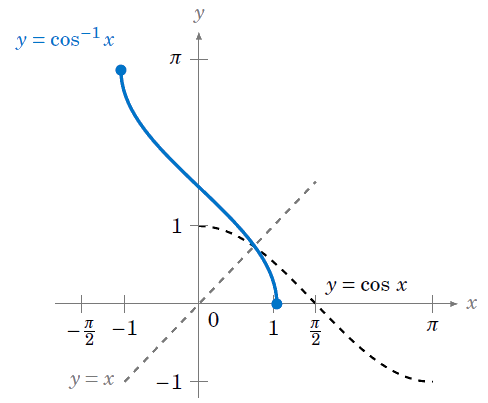
\includegraphics[width=0.45\textwidth]{Last.png}
    \caption{The curve y = arccos x}
\end{figure}

\textbf{Properties of arccosine}\\
For the arccosine function to be a true inverse function of the sine function, the following statement must be true: cos (arccos (x))  =   x   and   arccos (cos (x))  =  x\\
The arccosine function is a reflection of the cosine function about the line y = x.\\
The function  arccosine  is defined on the interval [-1,1] and are continuous on the open interval (-1,1).

\textbf{Application of function}\\
Arccosine function are unique function and useful in finding remaining two angles of right triangle.

\textbf{References}\\
https://en.wikipedia.org/wiki/Inverse\textunderscore trigonometric\textunderscore functions\\
https://courses.lumenlearning.com/boundless-algebra/chapter/trigonometric-functions-and-the-unit-circle/
\end{document}